\documentclass[lang=cn,10pt]{elegantbook}

\title{Complex Analysis}
% \subtitle{Elegant\LaTeX{} 经典之作}

\author{Lollins}
% \institute{Elegant\LaTeX{} Program}
\date{\today}
% \version{4.3}
% \bioinfo{自定义}{信息}

\extrainfo{改变人生的事情,你必须冒险;
意义非凡的事情,大多碰巧发生;
不重要的事,才有周全的计划。
}

\setcounter{tocdepth}{3}

\logo{logo.jpg}
\cover{star.jpg}

% 本文档命令
\usepackage{array}
\newcommand{\ccr}[1]{\makecell{{\color{#1}\rule{1cm}{1cm}}}}

% 修改标题页的橙色带
\definecolor{customcolor}{RGB}{135, 206, 235}
\colorlet{coverlinecolor}{customcolor}
\begin{document}

\maketitle

\begin{center}
	\Huge\textbf{前言}
\end{center}~\

$2023/8/11$,第一次拿\LaTeX 做数学笔记,用这份Note记录一些学习复变的过程中遇到的小知识点。

$2023/9/6$,今天从网上看到了这份$ElegantBook$,刚好这个学期学习复变,修改一下暑假做的这份零碎笔记。
~\\
\begin{flushright}
	\begin{tabular}{c}
		Lollins \\
		\today
	\end{tabular}
\end{flushright}


\frontmatter

\tableofcontents

\mainmatter




\chapter{Complex Number}
\begin{introduction}
	\item 复数的基本运算
	\item 平方根
	\item 共轭
	\item 绝对值(模)
	\item 不等式
\end{introduction}

\section{算数运算}








\appendix
\chapter{Topology}
\begin{introduction}
	\item 点集
	\item 区域
	\item 曲线
\end{introduction}

\section{点集}
\begin{definition}[邻域]
	设$\alpha \in \mathbf{C},r \in (0,\infty)$。集
	\begin{equation}
		\{z:\mid z-\alpha\mid<r,z\in\mathbf{C}\}
	\end{equation}
	称为以$\alpha$为中心、$r$为半径的圆盘,$\text{或者称为}$$\alpha\text{的一个邻域或}r$邻域
		,记作$U(\alpha,r)$。
\end{definition}

\begin{definition}[聚点]
	如果$\forall r >0,U(\alpha,r) \cap \mathbf{E}$中有无穷个点,那么$\alpha$称为集$\mathbf{E}$
	的一个聚点或者极限点;这时它可能属于集$\mathbf{E}$,也可能不属于。
\end{definition}

\begin{definition}[内点]
	如果$\exists r >0,$使得$U(\alpha,r) \subset \mathbf{E}$,那么$\alpha$称为集$\mathbf{E}$
	的内点;它显然是属于集$\mathbf{E}$的,并且为聚点。
\end{definition}

\begin{definition}[边界点]
	如果$\forall r >0,U(\alpha,r)\cap \mathbf{E}\neq\varnothing,U(\alpha,r)\cap\complement \mathbf{E}\neq\varnothing $,
	那么$\alpha$称为集$\mathbf{E}$的边界点。
\end{definition}

\begin{definition}[边界]
	集$\mathbf{E}$的全部边界点组成的集,称为集$\mathbf{E}$的边界,记作$\partial\mathbf{E}$。$\partial\mathbf{E}$中的点
	不一定属于集$\mathbf{E}$,也不一定是集$\mathbf{E}$的聚点,参考图\ref{imA_1}。
\end{definition}

\begin{figure}[h]
	\centering
	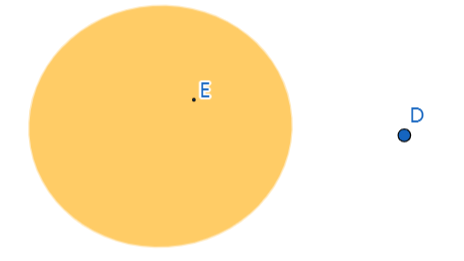
\includegraphics[scale = 0.6]{image/A_1.png}
	\caption{图中$D \in \mathbf{E}$为集$\mathbf{E}$的边界点,但不是聚点}
	\label{imA_1}
\end{figure}

\begin{definition}[闭包]
	$\mathbf{E}\cup\partial \mathbf{E}$称为集$\mathbf{E}$的闭包,记作$\mathbf{\overline E}$。
\end{definition}

\begin{definition}[孤立点]
	如果$\exists r >0,$使得$U(\alpha,r) \cap \mathbf{E} = \{\alpha\}$,那么$\alpha$是集$\mathbf{E}$
	的一个边界点,但不是聚点,它称为孤立点。
\end{definition}

\begin{definition}[开集]
	如果集 $\mathbf{E}$ 中的点全部是内点,那么集 $\mathbf{E}$ 称为开集。
\end{definition}

\begin{definition}[闭集]
	如果集$\mathbf{E}$或者没有聚点,或者所有聚点都属于集$\mathbf{E}$,那么集$\mathbf{E}$称为闭集;任何集 $\mathbf{E}$ 的闭包 $\overline{\mathbf{E}}$必然是一闭集。
\end{definition}

\begin{definition}[有界集与无界集]
	如果$\exists r >0,$使得$U(\alpha,r) \supset \mathbf{E}$,那么集$\mathbf{E}$称为有界集;
	否则称集$\mathbf{E}$为无界集。
\end{definition}

\begin{definition}[紧集]
	复平面$\mathbf{C}$上的有界闭集称为紧集。
\end{definition}

\section{区域}
\begin{definition}[区域]
	复平面$\mathcal{C}$上具有下列性质的点击$D$称为区域:
	\begin{enumerate}
		\item $D$是开集;
		\item $D$中任意两个有限点可以用有限个相衔接的线段所构成的折线连结起来,
		      而使这个折线上的点完全属于$D$
	\end{enumerate}
	如果区域$D$是有界集,那么它就称为有界区域;否则称为无界区域。
\end{definition}

性质2称为\textbf{连通性},简单的说,区域就是连通的开集。

\begin{definition}[闭区域]
	区域$D$内及其边界上全部点所组成的集称为闭区域,记作$\overline{D}$。按照$D$是否有界,可
	分为有界闭区域和无界闭区域。
\end{definition}

\section{曲线}
\begin{definition}[连续曲线·若尔当曲线]
	设已给
	\begin{equation}\label{eqA.2}
		z=z(t)\quad(a\leq t \leq b)
	\end{equation}
	在这里Re$~z(t)$及Im$~z(t)$都在闭区域$[a,b]$上连续。集$\left\{z(t):t\in\left[a,b\right]\right\}$
	称为一条连续曲线,记作\ref{eqA.2}。

	如果对$[a,b]$上任意两个不同点$t_1,t_2$,但不同时是$[a,b]$的端点,我们有$z(t_1)\neq z(t_2)$,
	那么式\ref{eqA.2}称为一条简单连续曲线,或若尔当曲线。如果还有$z(a)= z(b)$,式\ref{eqA.2}称为一条简单连续闭合曲线,或若尔当闭合曲线。
\end{definition}

\begin{definition}[连通区域]
	在复平面$\mathbf{C}$上,如果区域$D$内任何简单封闭曲线的内区域中每一点都属于$D$,那么称
	$D$为单连通区域;不是单连通的区域,称为多连通区域,参考图\ref{imA_2}。
\end{definition}

\begin{figure}[h]
	\centering
	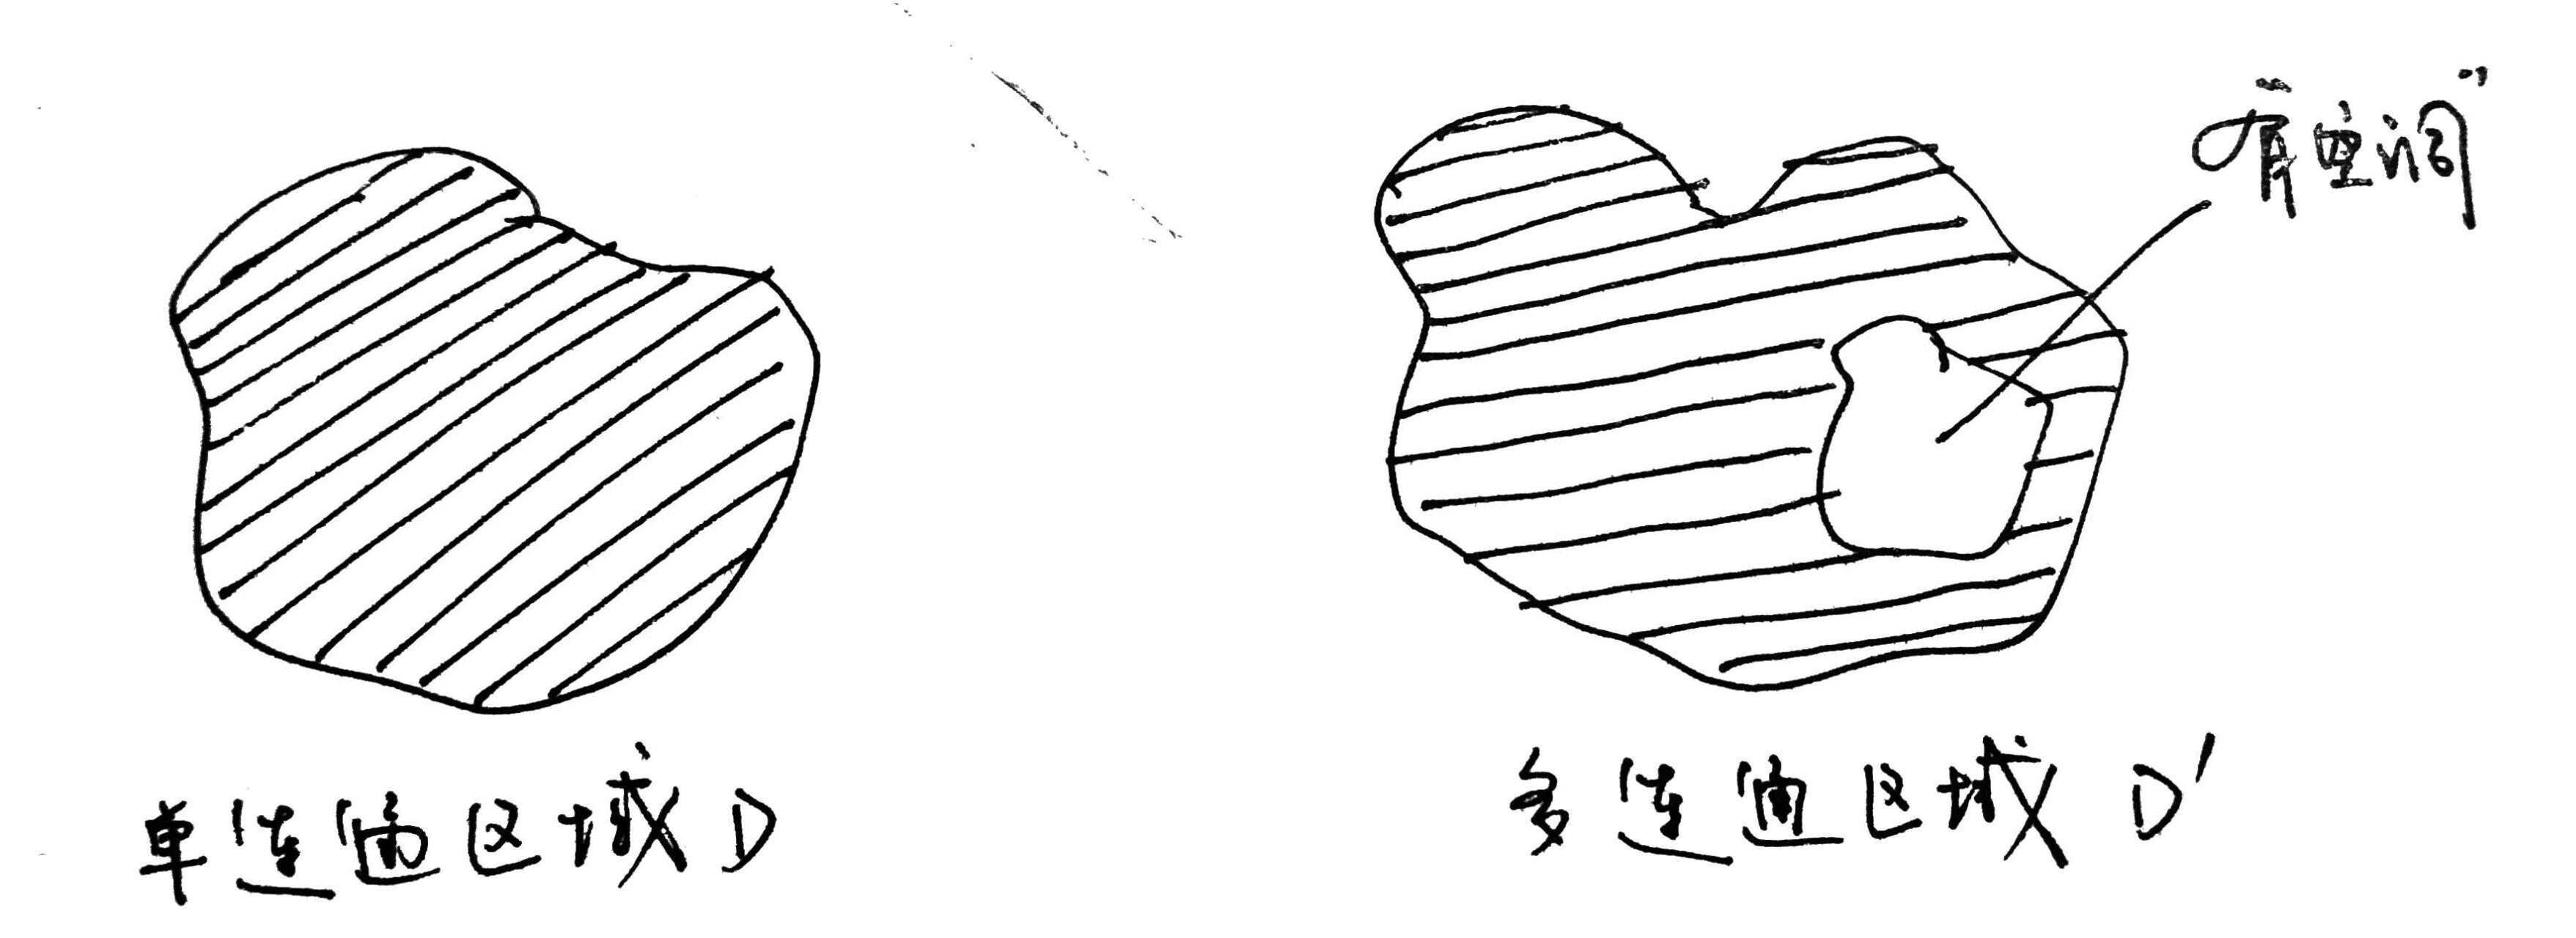
\includegraphics[scale=0.1]{image/A_2.jpg}
	\caption{}
	\label{imA_2}
\end{figure}


\end{document}